\documentclass[a4paper, 10pt, final, garamond]{book}
\usepackage{cours-preambule}

\makeatletter
\renewcommand{\@chapapp}{M\'ecanique -- chapitres}
\makeatother

\hfuzz=5.002pt

% \toggletrue{student}
\toggletrue{corrige}
% \renewcommand{\mycol}{black}
\renewcommand{\mycol}{gray}

\begin{document}
\setcounter{chapter}{7}

% \settype{enon}
% \settype{solu_prof}
% \settype{solu_stud}

\chapter{TD~: moment cin\'etique et forces centrales}

\section{Levier}
\textsc{Archimède} (240 av. J.-C.) est le premier à établir la théorie physique
du levier et de la balance. Il aurait dit~: «~Donnez-moi un point fixe et un
levier, et le soulèverai la Terre~».
\smallbreak
Imaginons une situation pour réaliste où \textsc{Archimède} utilise un levier
afin de soulever un rocher de masse $M = \SI{200}{kg}$. Les longueurs sont $d_1
	= \SI{50}{cm}$, $d_2 = \SI{1.5}{m}$ et $\alpha = \ang{60}$.
\begin{figure}[htbp!]
	\centering
	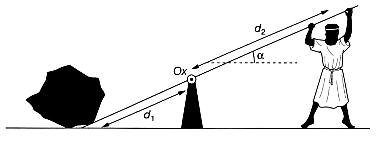
\includegraphics[width=.7\linewidth]{archi_plain-white}
	\label{fig:bld_1}
\end{figure}
\QR{%
	\textsc{Archimède se suspend verticalement au levier. Quelle doit être sa
		masse minimale pour que le rocher se soulève~?}
}{%
	solu
}
\QR{%
	\textsc{Archimède} décide de faire varier la direction de la force qu'il
	exerce sur le levier sans changer sa norme. Comment doit-il procéder pour être
	le plus efficace~? Quel est le gain par rapport au cas précédent~?
}{%
	solu
}

\section{Pendule pesant non amorti}
Une benne de téléphérique, de masse $M = \SI{2.0e3}{kg}$, est accrochée au point
A situé à l'extrémité inférieure d'un bras de masse $m = \SI{300}{kg}$ relié à
des câbles au point O. On note $a = \SI{4.5}{m}$ la distance entre O et G le
centre de gravité de l'ensemble \{benne+bras\}, situé sur l'axe (OA).
\smallbreak
On note $J\ind{tot}$ le moment d'inertie de l'ensemble par rapport à l'axe de
rotation $y$, et la liaison est supposée parfaite. On effectue un test
d'oscillations de la benne, le point O étant maintenant fixe.
\QR{%
	En appliquant le théorème du moment cinétique, déterminer l'équation
	différentielle vérifiée par $\th$.
}{%
	solu
}
\QR{%
	En déduire la période $T$ des petites oscillations de la benne.
}{%
	solu
}
\QR{%
	Sachant que la période des petites oscillations est $T = \SI{4.1}{s}$ et que
	le bras de longueur $L = \SI{3.0}{m}$ a un moment d'inertie $J' =
		\frac{1}{3}mL^2$ par rapport à l'axe $y$, calculer le moment d'inertie $J$ de
	la benne par rapport à $y$. On rappelle que $g = \SI{9.81}{m.s^{-2}}$ et on
	indique que dans ce cas, les moments d'inertie se somment.
}{%
	solu
}

\section{Chute d'un arbre}
\noindent
\begin{minipage}[c]{.70\linewidth}
	On étudie la chute d'une arbre~: on souhaite connaître la durée que met l'arbre,
	une fois tranché ç sa base, pour tomber au sol.
	\smallbreak
	On modélise la situation par une tige homogène de hauteur $L = \SI{10}{m}$ et de
	masse $m$, reliée au sol par une liaison pivot parfaite et qui part d'un angle
	initial $\th_0 = \SI{1.5}{rad}$ avec une vitesse initiale nulle. On donne le
	moment d'inertie par rapport à O$z$~: $J_z = \frac{1}{3}mL^2$.
\end{minipage}
\hfill
\begin{minipage}[c]{.25\linewidth}
	~
	\begin{center}
		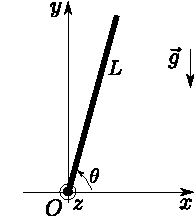
\includegraphics[width=\linewidth]{arbre_plain.pdf}
		\label{fig:arbre_chute}
	\end{center}
\end{minipage}

\QR{%
	Donner les expressions des énergies cinétique et potentielle de pesanteur de
	l'arbre.
}{%
	solu
}
\QR{%
	Justifier que l'énergie mécanique est constante au cours du mouvement.
	Exprimer cette constante en utilisant les conditions initiales.
}{%
	solu
}
\QR{%
	En déduire la relation
	\[
		\dv{\th}{t} = - \sqrt{\frac{3g}{L}(\sin{\th_0} - \sin{\th})}
	\]
}{%
	solu
}
\QR{%
	Retrouver ce résultat par le TMC.
}{%
	solu
}
\QR{%
	Pour exprimer la durée $T$ de la chute, isoler $\dd{t}$ dans l'expression
	précédente puis l'intégrer entre $\th = \th_0$ et $\th = 0$. Faire
	l'application numérique, sachant que $\DS
		\int_{0}^{\th_0}\frac{\dd{\th}}{\sqrt{\sin{\th_0} - \sin{\th}}} \approx
		\num{5.44}$ pour $\th_0 = \SI{1.5}{rad}$.
}{%
	solu
}
\QR{%
	\textit{Bonus} Écrire un script \texttt{Python} permettant de calculer
	numériquement l'intégrale précédente.
}{%
	solu
}

\section{Barre fixée à ses extrémités}
\noindent
\begin{minipage}[c]{.70\linewidth}
	Considérons le système mécanique représenté ci-contre, constitué d'une barre
	homogène de masse $m$, de longueur OA $= 2a$, libre de tourner sans frottement
	autour de l'axe O$z$ (liaison parfaite). Son moment d'inertie par rapport à
	cet axe vaut $J_z = \frac{4}{3}ma^2$. Elle est attachée en A à un ressort de
	longueur à vide $\ell_0$ et de raideur $k$. L'autre extrémité du ressort est
	fixe.
\end{minipage}
\hfill
\begin{minipage}[c]{.25\linewidth}
	~
	\begin{center}
		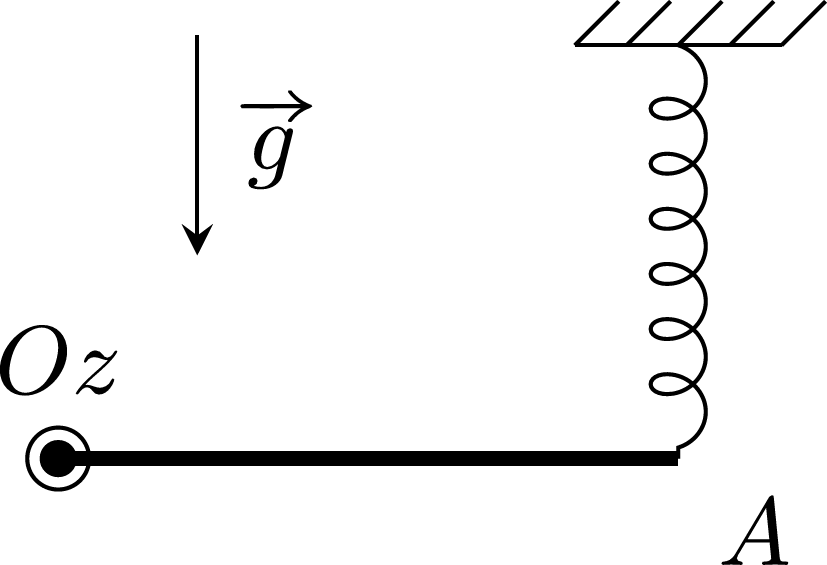
\includegraphics[width=\linewidth]{brr_fixe-plain}
	\end{center}
\end{minipage}
\QR{%
	À l'équilibre, las barre est horizontale et le ressort vertical. En déduire la
	longueur du ressort à l'équilibre en fonction de $k, \ell_0, m$ et $g$.
}{%
	\begin{center}
		\includegraphics[width=\linewidth]{brr_fixe-corr}
	\end{center}

}
\QR{%
	La barre est légèrement écartée de sa position d'équilibre, puis lâchée sans
	vitesse initiale. Déterminer la période des petites oscillations. Comme les
	angles sont très petits, on peut considérer que le point A se déplace
	verticalement.
}{%
	solu
}

\section{Choc de deux chariots}
\noindent
\begin{minipage}[c]{.45\linewidth}
	Deux masses $m_1$ et $m_2$ sont montées sur un banc horizontal à coussins
	d'air, de sorte qu'on peut négliger tout frottements. On les projette l'une
	contre l'autre avec des vitesses initiales $\vf_1 = v_1 \ux$ et $\vf_2 =
		\of$ ($m_2$ initialement à l'arrêt).
\end{minipage}
\hfill
\begin{minipage}[c]{.45\linewidth}
	~
	\begin{center}
		\includegraphics[width=\linewidth]{chariots_plain}
	\end{center}
\end{minipage}
\begin{blocQR}
	\item \textit{Dans cette partie, on suppose qu'après le choc les masses
		restent solidaires.}
	\QR{%
		Quelle est la vitesse commune des deux masses après le choc~?
	}{%
		solu
	}
	\QR{%
		Quel est le travail des actions intérieures lors du choc~? Commenter le
		signe du résultat.
	}{%
		solu
	}
\end{blocQR}
\begin{blocQR}
	\item \textit{On considère dans cette partie que le choc est élastique,
		c'est-à-dire que l'énergie cinétique de l'ensemble des deux masses est
		conservée au cours du choc et qu'elles ne sont plus solidaires après.}
	\QR{%
		Montrer que les vitesses $v_1'$ et $v_2'$ après le choc s'expriment~:
		\[
			v_1' = \frac{m_1-m_2}{m_1+m_2}v_1
			\qet
			v_2' = \frac{2m_1}{m_1+m_2}v_1
		\]
	}{%
		solu
	}
	\QR{%
		Que se passe-t-il si $m_2 \gg m_1$~?
	}{%
		solu
	}
	\QR{%
		À quelle condition sur $m_1$ et $m_2$ est-il possible de réaliser un
		«~carreau~», i.e.\ échanger lors du choc les vitesses des deux masses,
		comme à la pétanque~?
	}{%
		solu
	}
\end{blocQR}

\section{Étagère murale}
\noindent
\begin{minipage}[c]{.45\linewidth}
	Une étagère est suspendue par quatre câbles métalliques et fixée au mur
	uniquement par deux pattes de fixation murale (en A et A'). La planche est en
	bois, de masse $m = \SI{1.0}{kg}$, de centre de masse G situé à la distance
	$R/2$ de l'axe (OO') et nous négligerons la masse des câbles.
\end{minipage}
\hfill
\begin{minipage}[c]{.45\linewidth}
	~
	\begin{center}
		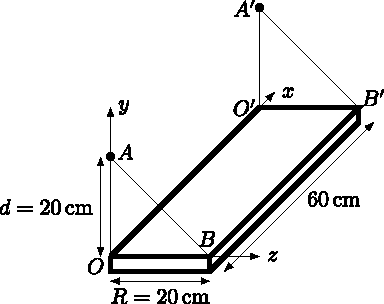
\includegraphics[width=\linewidth]{etg_plain.pdf}
	\end{center}
\end{minipage}

\QR{%
	Exprimer les 4 forces de tension des câbles et la force de réaction $\Rf_n$ du
	mur sur la planche lorsque l'étagère est posée et en équilibre. $\Rf_n$ est
	supposée normale au mur. Calculer les valeurs numériques des normes des
	forces.
}{%
	solu
}
\QR{%
	On imagine que les 2 câbles fixés en B et B' se rompent en même temps. La
	planche n'est alors retenue que par les câbles OA et OA', et elle tourne donc
	autour de l'axe $\D = (\rm OO')$. Nous négligerons sont épaisseur et
	admettrons que son moment d'inertie par rapport à l'axe $\D$ vaut $J_{\D} =
		mR^2$. Montrer qu'alors~:
	\[
		\tp^2 = \frac{mgR}{J_{\D}}\sin(\th)
	\]
	En déduire la vitesse angulaire de la planche lorsqu'elle percute le mur.
}{%
	solu
}

\section{Entraînement par frottements}
\noindent
\begin{minipage}[c]{.48\linewidth}
	On considère le système de deux disques en rotation, de moments d'inertie
	$J_1$ et $J_2$ par rapport à l'axe horizontal orienté par $\uz$. Ils sont tous
	les deux en liaison pivot parfaite. Le second disque a une vitesse angulaire
	$\w_0$, alors que le premier est initialement immobile. On translate
	lentement les disques le long de l'axe jusqu'à ce qu'ils rentrent en contact.
	Il n'y a plus de frottement après la mise en contact.
\end{minipage}
\hfill
\begin{minipage}[c]{.48\linewidth}
	~
	\begin{center}
		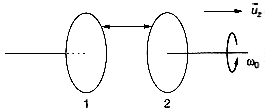
\includegraphics[width=\linewidth]{entr_frott-plain-white}
	\end{center}
\end{minipage}
\QR{%
	À quelle condition sur les vitesses angulaires n'y a-t-il plus de
	frottements~? Déterminer alors les vitesses angulaires finales de deux disques
	par application du TMC sur le système total.
}{%
	solu
}
\QR{%
	Faire un bilan d'énergie pour chaque disque séparément.
}{%
	solu
}
\QR{%
	Faire le même bilan pour le système total.
}{%
	solu
}
\QR{%
	Commenter les résultats.
}{%
	solu
}

\section{Expérience de \textsc{Cavendish}}
L'expérience réalisée par \textsc{Cavendish} en 1789 a permis à ce dernier
d'obtenir une valeur remarquable de la constante de gravitation universelle,
$\Gc$. Le dispositif est constitué de deux petites sphères, de masse $m =
	\SI{0.72}{kg}$, fixées aux extrémités d'une tige de masse négligeable, rigide,
et longueur $\ell = \SI{180}{cm}$ et suspendue horizontalement, en son milieu, à
un fil de torsion vertical et très fin de constante de torsion $C$~: si la tige
tourne d'un angle $\th$ par rapport à sa position d'équilibre $\th = 0$, le fil
exercice ainsi le couple de rappel $\vv{\G} = -C\th \uz$ sur la tige.
\smallbreak
Deux boules de plomb de masse $M = \SI{160}{kg}$ sont fixées, l'une derrière une
petite sphère et l'autre devant l'autre petite sphère, à une distance $r =
	\SI{20}{cm}$ définie sur le schéma ci-dessous. Les deux forces d'attraction
gravitationnelle produisent un couple qui fait tourner la tige d'un angle $\th$
par rapport à sa position au repos. Les deux petites sphères se rapprochent
ainsi des boules de plomb jusqu'à ce que la torsion du fil s'équilibre avec le
couple gravitationnel.
\begin{figure}[htbp!]
	\centering
	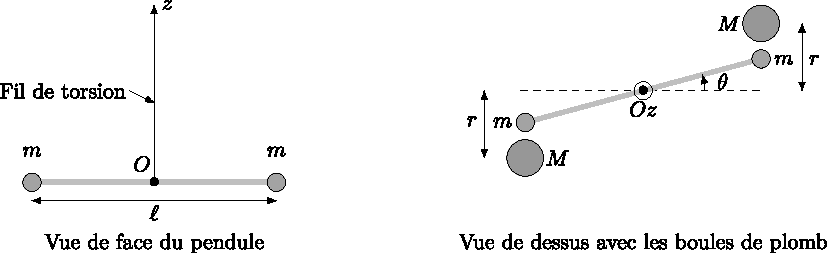
\includegraphics[width=.8\linewidth]{cav_plain}
\end{figure}
\begin{blocQR}
	\item Nous cherchons dans un premier temps à déterminer la constante de
	torsion $C$ du pendule en faisant osciller celui-ci. Les boules en plomb ne
	sont pas encore présentes.
	\QR{%
		Montrer à l'aide du TMC que l'oscillateur est harmonique, de pulsation
		propre $\w_0 = \sqrt{\frac{2C}{m \ell^2}}$.
	}{%
		solu
	}
	\QR{%
		La mesure de la période $T_0$ des oscillations donne $T_0 =
			\SI{7.0}{min}$. En déduire la valeur de $C$.
	}{%
		solu
	}
\end{blocQR}
\QR{%
	Les boules étant placées, déterminer l'expression de la déviation angulaire
	$\th$ par rapport à la position d'équilibre. On tiendra compte du fait que
	$\th$ est extrêmement faible pour évaluer le couple exercé par les deux
	boules de plomb.
}{%
	solu
}
\QR{%
La valeur obtenue par \textsc{Cavendish} à l'aide de ce dispositif et $\Gc =
	\SI{6.75e-11}{N.m^2.kg^{-2}}$. En déduire la déviation angulaire et commenter.
}{%
solu
}

\end{document}
